\exercise{Drawing the Mandelbrot fractal set}

\paragraph{Explanation:}
I have structured the code in several functions in order to keep it organized.
The first and main function is the \mttext{mandel} function, which starts out the location cache (in order to go back later if wanted) and the loop to listen to user inputs.

Then, there is the \mttext{compute\_mandel} which returns a matrix with the final values of the algorithm found in the problem set statement.
Two improvements have been made, a) writing into \mttext{V(i,j)} only once and b) checking wether \mttext{V(i,j)} has been set before computing iteration.
Additionally, I have created a base mask where if there is an overlap between the last saved computation and the current, then the previous will be set.
This will be especially handy for the ``vi motions'' I have implemented, saving computation time.
I have recently started learning and using these motions and thought it would be nice to implement the basic \textit{h,j,k,l} motions.
You can find a motions cheat sheet \href{https://vim.rtorr.com}{here}.
Next, there is \mttext{plot\_mandel}, which as the name suggests makes the image and outputs it as well as the text seen in the results section.
For some extra color I added a \textit{scaling factor} to multiply the final calculation by.
This added contrast to the plot making it a bit nicer in my opinion.

Finally, there is the \mttext{user\_input} function, which has the the mouse click to select a region as well as the following implemented,
\begin{itemize}
    \item \textit{quitting}: pressing \textit{q} or \textit{Q}
    \item \textit{iterations}: pressing \textit{+} or \textit{-} to increase or decrease them 
    \item \textit{undo}: pressing \textit{u} we can go back to the previous X,Y ranges, this was implemented by saving all the selected regions in a variable called \mttext{cache}
    \item \textit{points}: pressing \textit{X} or \textit{x} to increase or decrease the x axis points, same goes for \textit{Y} and \textit{y} for the y axis
    \item \textit{scaling factor}: pressing \textit{S} or \textit{s} to increase or decrease it
    \item \textit{motions}: pressing \textit{h} to go to the left, \textit{j} to go down, \textit{k} to go up and \textit{l} to go right
    \item \textit{zooming}: finally, I also implemented the option to zoom in and out by pressing \textit{spacebar} followed by \textit{+} or \textit{-}

\end{itemize}

All the increases are done by a factor defined in the \mttext{user\_input} function.

\paragraph{MATLAB Code:}

\begin{tiny}
    \verbatiminput{code/mandelbrot.m}
\end{tiny}

\paragraph{Results:}

\begin{figure}[H]
    \centering
    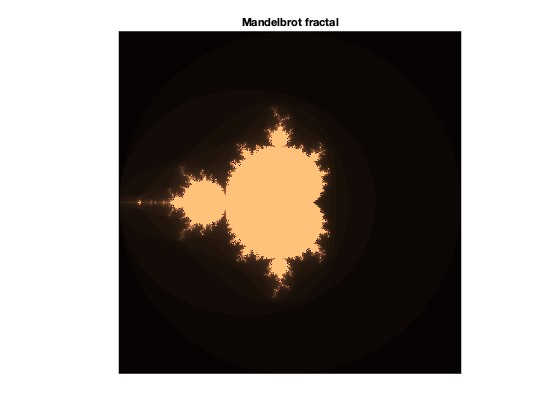
\includegraphics[width=8cm]{figures/base}
    \caption{Base plot}
\end{figure}
\begin{verbatim}
==================================
Mandelbrot fractal at
    X: [-2.000000000, 2.000000000]
    Y: [-2.000000000, 2.000000000]
    Iterations:                100
    Scaling factor:              5
    Points:            500  x  500
==================================
\end{verbatim}

\begin{figure}[H]
    \centering
    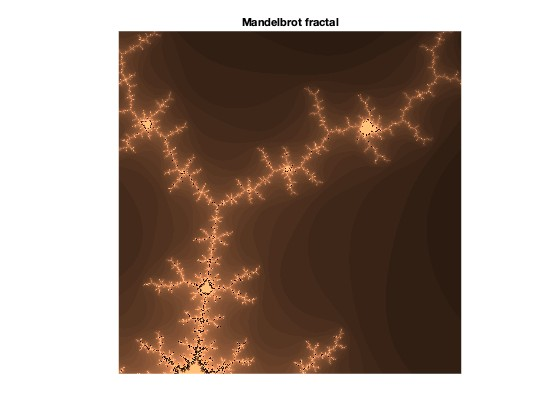
\includegraphics[width=8cm]{figures/main}
    \caption{Example plot}
\end{figure}

\begin{verbatim}
==================================
Mandelbrot fractal at
    X: [-0.138997555, -0.007315661]
    Y: [0.891799511, 1.023481405]
    Iterations:                100
    Scaling factor:              5
    Points:           1688  x 1688
==================================
\end{verbatim}

\begin{figure}[H]
    \centering
    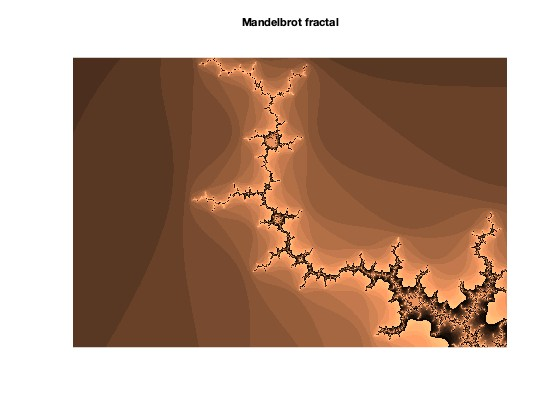
\includegraphics[width=8cm]{figures/scaled}
    \caption{Scaled shenanigans}
\end{figure}

\begin{verbatim}
==================================
Mandelbrot fractal at
    X: [-1.352398048, -1.141634716]
    Y: [0.421526664, 0.281017776]
    Iterations:                100
    Scaling factor:             12
    Points:           2532  x 1125
==================================
\end{verbatim}


\begin{figure}[H]
    \centering
    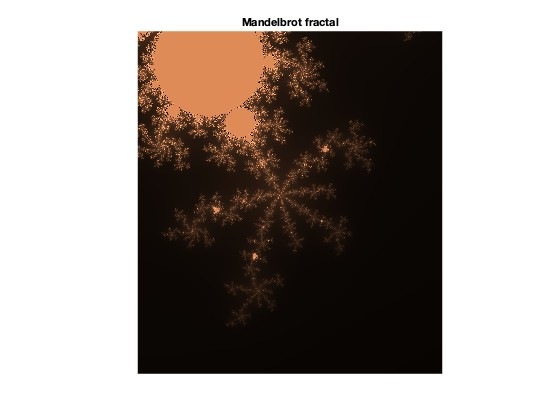
\includegraphics[width=8cm]{figures/max}
    \caption{Computation at the limit}
\end{figure}

\begin{verbatim}
==================================
Mandelbrot fractal at
    X: [0.099527129, 0.193199721]
    Y: [-0.601846404, -0.707228070]
    Iterations:               1713
    Scaling factor:              1
    Points:           1125  x 1125
==================================
\end{verbatim}


\paragraph{Comments:}
It is possible I ended up obscuring the code a bit (due to some of the optimisations I implemented), but I have tried my best to add comments where necessary to explain the weirdest parts as well as naming functions and variables for what they do.
Some tricky issues I ran into was setting up the motions and zoom in/out right, as calculating the movement value was being affected by what quadrant I was in, so I ended up using the \mttext{abs} function for the motions.
Additionally, I am not incredibly happy with the final colors of my plot and would have also liked to work on a legend, but I spent too much time figuring out all the user inputs.
Aside from that it was a fun exercise, one of the main reasons being that I had never computed the Mandelbrot fractal!
